\section{DataBean und DataProxy} \label{chp:data}
Input und Output der einzelnen \name{Steps} ist ein einziges
Datenobjekt vom Typ \code{DataBean}. 
\index{DataBean}
\index{Klasse!DataBean}
\code{DataBean} ist nach dem Konzept der \name{JavaBeans\texttrademark}
\footnote{
JavaBeans\texttrademark ist ein \name{Komponentenmodel} \seec{chp:osgi} für
Java, das grundsätzlich folgende Eigenschafften an einzelne Klassen
(\name{beans}) stellt: \textbf{Öffentlicher Standardkonsstruktor},
\textbf{Öffentliche \name{getter} und \name{setter} methoden},
\textbf{Implementierung des \name{Serializable} Interface}
\citep{beans_1997}
}
entworfen und ist mit hierfür typischen Funkionalitäten wie Serialisierung und
öffentlichen  \name{getter} und \name{setter} Methoden ausgestattet.
\index{JavaBean}

\name{DataBean} bietet den Steps der Pipeline die Möglichkeit, ihre
(Zwischen-)Ergebnisse zentral abzuspeichern.
Die zu annotierende Inputsequenz ist dabei ebenfalls Teilmenge der
von \name{DataBean} gespeicherten Daten.

Da es nur ein einziges Objekt vom Typ \code{DataBean} geben soll, das zentral
und für jeden Step innerhalb der Pipeline verfügbar ist, wird der Zugriff auf
dieses Objekt an einen Proxy
\footnote{
Der \first{Proxy}, oder auch \first{Stellvertreter} ist ein Entwurfsmuster
\seec{chp:softwarearchitektur}, das eine Klasse beschreibt, die als (alleinige)
Schnittstelle zu einem anderen Objekt auftritt.
Als Stellvertreter dieses Objekts kann der Proxy die Erzeugung des Subjektes
sowie den Zugriff darauf kontrollieren.
\citep{freeman_entwursmuster_2005, gamma_entwurfsmuster:_2009}
}
delegiert. Dieser übernimmt zudem die Implementierung einer geeigneten
Serialisierungsstrategie und synchronisiert die Zugriffe auf das
\name{DataBean}.

Durch den Proxy ist die kongrekte Implementierung der Datenpersistierung vom
Rest der Pipeline getrennt und kann leicht verändert werden.
So wäre es beispielsweise denkbar, die Daten nicht local in einer Binärdatei
abzuspeichern, sondern entfernt in einer Datenbank abzulegen.

Der \name{DataProxy} ist wie das \name{DataBean} innerhalb der Pipeline ein
\name{Singleton}
\footnote{Unter dem Entwurfsmuster \seec{chp:softwarearchitektur} des
\first{Singleton} versteht man eine Klasse, von der nicht mehr als ein einziges
Objekt erstellt werden kann.
Das Objekt dieser Klasse ist in der Regel global verfügar.
\citep{freeman_entwursmuster_2005, gamma_entwurfsmuster:_2009}
}.
Eine Referenz auf \name{DataProxy} ist Input für jeden Step und enthält nach
dessen Ausführung auch die gewonnenen Ergebnisse.

\begin{figure}[htbp]
	\begin{center}
		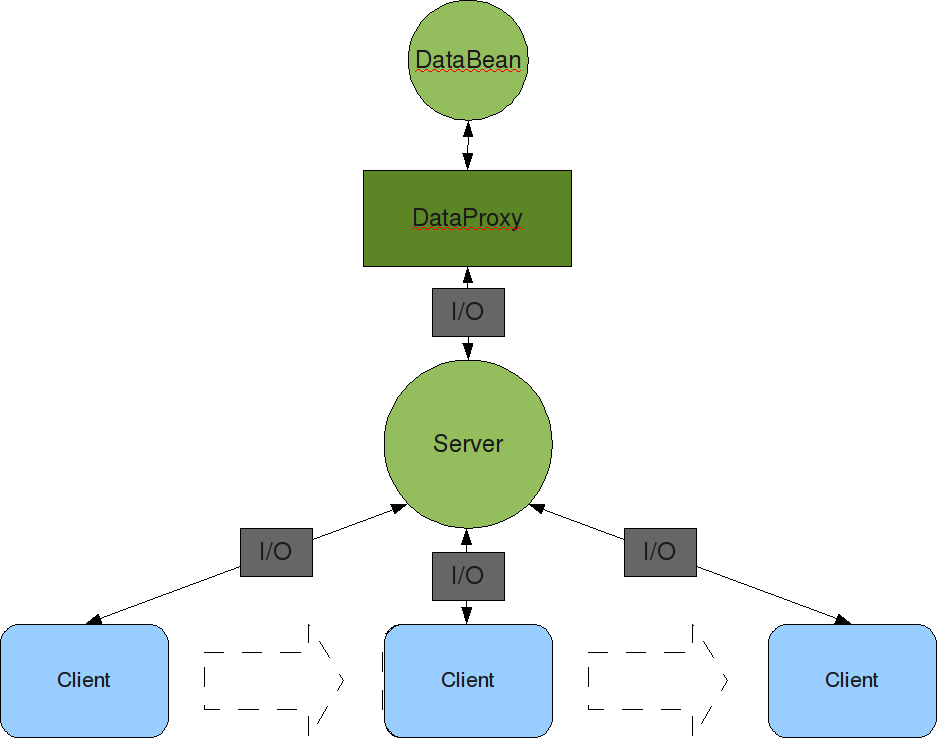
\includegraphics[scale=0.55]{pics/serverClientData2.png}
	\caption[\name{DataProxy} im Client-Server Pattern]{
	\textbf{\name{DataProxy} im Client-Server Pattern.}
	}
	\end{center}
	\label{fig:pipesFilter41}
\end{figure}

\begin{figure}[htbp]
	\begin{center}
		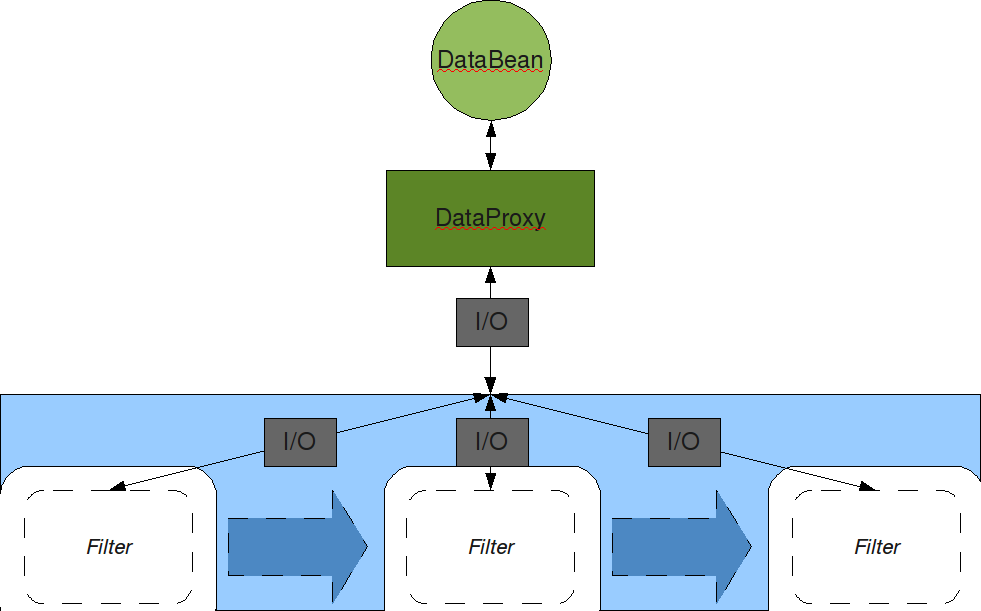
\includegraphics[scale=0.55]{pics/pipesFilter41.png}
	\caption[\name{DataProxy} im Pipes and Filters Pattern]{
	\textbf{\name{DataProxy} im Pipes and Filters Pattern.}
	}
	\end{center}
	\label{fig:pipesFilter41}
\end{figure}

